\documentclass[a4paper]{article}
%\documentclass[a4paper,fontsize=13pt]{scrartcl}

\author{Huỳnh Sâm Hà - 1610852@hcmut.edu.vn}

\usepackage{vntex}
%\usepackage{helvet} %set font Helvetica
%\usepackage{times} %set font Times New Roman
\renewcommand{\familydefault}{\sfdefault} %set font Sans Serif

%%%%% change language vietname - english
%\usepackage[english,vietnam]{babel}
%\usepackage[utf8]{inputenc}
%\usepackage[francais]{babel}

\usepackage{a4wide,amssymb,epsfig,latexsym,array,hhline,fancyhdr}
\usepackage{amsmath}
\usepackage{amsthm}
\usepackage{multicol,longtable,amscd}
\usepackage{diagbox} %Make diagonal lines in tables
\usepackage{booktabs}
\usepackage{alltt}
\usepackage[framemethod=tikz]{mdframed} % For highlighting paragraph backgrounds
\usepackage{caption,subcaption}
\usepackage{lastpage}
\usepackage[lined,boxed,commentsnumbered]{algorithm2e}
\usepackage{enumerate}
\usepackage{color}
\usepackage{graphicx} % Standard graphics package
\usepackage{array}
\usepackage{tabularx, caption}
\usepackage{multirow}
\usepackage{rotating}
\usepackage{graphics}
\usepackage[left=2.5cm,right=2.5cm,top=2cm,bottom=3cm]{geometry} % margin page
\usepackage{a4wide,amssymb,epsfig,latexsym,array,hhline,fancyhdr}
\usepackage[makeroom]{cancel}
\usepackage{arydshln}
\usepackage{textcomp}
\usepackage{listings}
\usepackage{listingsutf8}
\usepackage{verbatim}

\usepackage{setspace}
%\singlespacing
%\onehalfspacing
%\doublespacing
%\setstretch{1.5}

\usepackage{epsfig}
\usepackage{tikz}
\usetikzlibrary{calc}
\newcommand\HRule{\rule{\textwidth}{1pt}}
\usetikzlibrary{arrows,snakes,backgrounds}
\usepackage[unicode]{hyperref}
\hypersetup{urlcolor=blue,linkcolor=black,citecolor=black,colorlinks=true} 
%\usepackage{pstcol} % PSTricks with the standard color package

\setlength\dashlinedash{1.5pt}
\setlength\dashlinegap{4.5pt}
\setlength\arrayrulewidth{0.2pt}

% Typesetting Listings
\usepackage{xcolor}
\usepackage{color}
\definecolor{listinggray}{gray}{0.9}
\definecolor{lbcolor}{rgb}{0.9,0.9,0.9}
\definecolor{Darkgreen}{rgb}{0.1,0.6,0.1}

\lstset{
	backgroundcolor=\color{lbcolor},
	tabsize=4,    
	%   rulecolor=,
	language=[GNU]C++,
	basicstyle=\scriptsize,
	upquote=true,
	aboveskip={1.5\baselineskip},
	columns=fixed,
	showstringspaces=false,
	extendedchars=false,
	breaklines=true,
	prebreak = \raisebox{0ex}[0ex][0ex]{\ensuremath{\hookleftarrow}},
	frame=single,
	numbers=left,
	showtabs=false,
	showspaces=false,
	showstringspaces=false,
	identifierstyle=\ttfamily,
	keywordstyle=\color[rgb]{0,0,1},
	commentstyle=\color[rgb]{0.026,0.112,0.095},
	stringstyle=\color[rgb]{0.627,0.126,0.941},
	numberstyle=\color[rgb]{0.205, 0.142, 0.73},
	%        \lstdefinestyle{C++}{language=C++,style=numbers}’.
}
\lstset{
	backgroundcolor=\color{lbcolor},
	tabsize=4,
	language=C++,
	captionpos=b,
	tabsize=3,
	frame=lines,
	numbers=left,
	numberstyle=\tiny,
	numbersep=5pt,
	breaklines=true,
	showstringspaces=false,
	basicstyle=\footnotesize,
	%  identifierstyle=\color{magenta},
	keywordstyle=\color[rgb]{0,0,1},
	commentstyle=\color{Darkgreen},
	stringstyle=\color{red}
}

%\usepackage{fancyhdr}
\setlength{\headheight}{40pt}
\pagestyle{fancy}
\fancyhead{} % clear all header fields
\fancyhead[L]{
	\begin{tabular}{rl}
		\begin{tabular}{l}
			\textbf{\bf HCMC University Of Technology - 
				Faculty of Computer Science \& Engineering}\\
		\end{tabular} 	
	\end{tabular}
}
\fancyhead[R]{
	\begin{tabular}{l}
		\tiny \bf \\
		\tiny \bf 
\end{tabular}  }
\fancyfoot{} % clear all footer fields
\fancyfoot[L]{\footnotesize Operating Systems - Assignment \#1-System Call}
\fancyfoot[R]{\footnotesize Trang {\thepage}/\pageref{LastPage}}
\renewcommand{\headrulewidth}{0.1pt}
\renewcommand{\footrulewidth}{0.1pt}

\setcounter{secnumdepth}{4}
\setcounter{tocdepth}{3}
\makeatletter
\newcounter {subsubsubsection}[subsubsection]
\renewcommand\thesubsubsubsection{\thesubsubsection .\@alph\c@subsubsubsection}
\newcommand\subsubsubsection{\@startsection{subsubsubsection}{4}{\z@}%
	{-3.25ex\@plus -1ex \@minus -.2ex}%
	{1.5ex \@plus .2ex}%
	{\normalfont\normalsize\bfseries}}
\newcommand*\l@subsubsubsection{\@dottedtocline{3}{10.0em}{4.1em}}
\newcommand*{\subsubsubsectionmark}[1]{}
\makeatother

\everymath{\color{blue}} %make in-line maths symbols blue to read/check easily

\sloppy
\captionsetup[figure]{labelfont={small,bf},textfont={small,it},belowskip=-1pt,aboveskip=-9pt}
%space remove between caption, figure, and text
\captionsetup[table]{labelfont={small,bf},textfont={small,it},belowskip=-1pt,aboveskip=7pt}
\setlength{\floatsep}{5pt plus 2pt minus 2pt}
\setlength{\textfloatsep}{5pt plus 2pt minus 2pt}
\setlength{\intextsep}{10pt plus 2pt minus 2pt}



\begin{document}

\begin{titlepage}

\begin{tikzpicture}[remember picture, overlay]
  \draw[line width = 3pt,color=blue] ($(current page.north west) + (2.2cm,-2.2cm)$) rectangle ($(current page.south east) + (-2.2cm,2.2cm)$);
   \draw[line width = 2pt,color=green] ($(current page.north west) + (2cm,-2cm)$) rectangle ($(current page.south east) + (-2cm,2cm)$);
\end{tikzpicture}
\vspace{0cm}
\begin{center} \large
TRƯỜNG ĐẠI HỌC BÁCH KHOA TP HCM \\
\textbf{KHOA KHOA HỌC VÀ KỸ THUẬT MÁY TÍNH } \\
- - - - - - - - - - - -
\end{center}


\vspace{1cm}
\begin{figure}[h!]
\begin{center}

\includegraphics[width=3.6cm]{Images/LogoBK}
\end{center}
\end{figure}
\vspace{1cm}



\begin{center}
\begin{tabular}{c}
\multicolumn{1}{c}{\textbf{{\huge KỸ NĂNG CHUYÊN NGHIỆP CHO KỸ SƯ}}}\\
~~\\
\hline
\\ \\
\multicolumn{1}{c}{\textbf{{\Large Báo cáo Bài tập nhóm}}}\\
\\
\textbf{{\Huge Đề xuất các giải pháp}} \\
\textbf{{\Huge về vấn đề trạm chờ xe buýt}} \\
\\ \\
\hline
\end{tabular}
\end{center}

\begin{table}[h]
\begin{tabular}{rrlrr}
\hspace{5cm} 
& Giáo viên hướng dẫn: & TS. Nguyễn Cao Trí & & \\ 
& Sinh viên thực hiện: & 1612212 - Nguyễn Trọng Nghĩa \\
&  & 1613535 - Nguyễn Văn Tiến\\
&  & 1610852 - Huỳnh Sâm Hà\\
&  & 1613575 - Trần Ngọc Tín\\
&  & 1612806 - Huỳnh Song Anh Quân\\
\end{tabular}
\end{table}

\vspace{2cm}

\begin{center}
{\footnotesize Tp. Hồ Chí Minh, Tháng 1/2018}
\end{center}

\end{titlepage}


\newpage \thispagestyle{empty} \tableofcontents
% \newpage \thispagestyle{empty} \listoftables
% \newpage \thispagestyle{empty} \listoffigures

\newpage

%%%%%%%%%%%%%%%%%%%%%%%%%%%%%%%%%%%%%%%%%%%
% set noindent all document
\setlength\parindent{0pt}
%%%%%%%%%%%%%%%%%%%%%%%%%%%%%%%%%%%%%%%%%%%

\section{Trạm dừng không được phân bố đồng đều dẫn đến khó khăn trong việc bắt xe bus.}

Giải pháp:

\begin{itemize}
	\item Đặt trạm ở vị trí thuận lợi.
	\item Thu hẹp khoảng cách giữa các trạm.
	\item Các trạm cần có bản đồ xe bus.
\end{itemize}




\section{Tình trạng kẹt xe ở trạm dừng gây khó khăn cho việc bắt xe, quá tải hành khách trên xe.}

Giải pháp:

\begin{itemize}
	\item Tăng cường số xe chạy trên các tuyến.
	\item Mở rộng qui mô trạm dừng để thuận tiện cho xe ra vào trạm, hành khách đón xe dễ dàng.
	\item Khi nhiều xe vào trạm, tài xế xe sau bị khuất tầm nhìn bởi xe trước, không biết hành khách đang chờ xe, khiến hành khách lỡ chuyến.
	\item Xây dựng làn đường riêng cho xe bus.
	\item Bố trí hợp lí thời gian xuất bến, cập bến các tuyến xe một cách hợp lí.
	\item Giải tán các điểm tụ tập buôn bán tại trạm dừng.
\end{itemize}

\section{Nhiều trạm không có chỗ ngồi, mái che, nhà vệ sinh công cộng gây khó khăn cho hành khách.}

Giải pháp:

\begin{itemize}
	\item Tăng không gian trạm dừng.
	\item Xây dựng nhà chờ có điều hòa, tránh mưa nắng tốt kết hợp với nhà vệ sinh công cộng.
\end{itemize}

\section{Vấn đề an ninh tại trạm dừng.}

Giải pháp:

\begin{itemize}
	\item Lập các đội bảo vệ gần trạm dừng.
	\item Lắp đặt camera.
\end{itemize}



\section{Hành khách không biết chính xác thời điểm xe tới.}

Giải pháp:

\begin{itemize}
	\item Lắp đặt bản đồ xe bus điện tử thông minh tại các trạm.
	\item Phát triển ứng dụng bản đồ thông minh trên các thiết bị di động cho người dùng.
	\item Lắp đặt biển báo dự kiến thời điểm xe vào trạm
\end{itemize}
%\section{Thiết kế, xây dựng hệ thống}

\subsection{Nền tảng và ngôn ngữ hiện thực}

\subsection{Thiết kế các cấu trúc dữ liệu}

\subsubsection{Hàng đợi ưu tiên \textit{(Priority Queue)}}

\paragraph{Mục đích sử dụng\\\\}

Quản lý hàng đợi các \textit{submission} cần được xử lý phía Server, với độ ưu tiên ở từng các \textit{submission}

\paragraph{Hiện thực\\\\}

Hình \ref{fig:class_priorityqueue} là lược đồ class của lớp PriorityQueue.

\begin{figure}[tph]
	\centering
	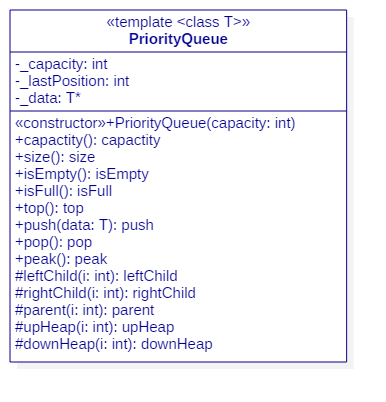
\includegraphics[width=8cm]{ClassDiagram/PriorityQueue}
	\vspace{0.3cm}
	\caption{Lược đồ class PriorityQueue}
	\label{fig:class_priorityqueue}
\end{figure}

\lstinputlisting{Code/pro-ass.xml}
%\section{Tổ chức và quản lý mã nguồn trong quá trình phát triển}

\subsection{Tổ chức và quản lý mã nguồn}

\subsection{Quản lý mã nguồn trên GitHub}
\textbf{Link GitHub:} \url{https://github.com/blabla}
%\section{Kiểm tra phần mềm}

\newpage


%%%%%%%%%%%%%%%%%%%%%%%%%%%%%%%%%
\addcontentsline{toc}{section}{Tài liệu tham khảo}
\begin{thebibliography}{99999}
	
\bibitem[medium.freecodecamp.org]{medium.freecodecamp.org} {
\href{https://medium.freecodecamp.org/building-and-installing-the-latest-linux-kernel-from-source-6d8df5345980}{How to build and install the latest Linux kernel from source?}}
	
\bibitem[man.he.net]{man.he.net} {
	\href{http://man.he.net/man5/kernel-package}{Document about kernel-package}}

\bibitem[cs.swarthmore.edu]{cs.swarthmore.edu} {
	\href{https://www.cs.swarthmore.edu/~newhall/unixhelp/howto_C_libraries.html}{Libraries in C}}


\bibitem[kernel.org]{kernel.org} {
	\href{https://www.kernel.org/doc/html/v4.12/process/adding-syscalls.html#x86-system-call-implementation}{Adding a New System Call - Compatibility System Calls}}


\end{thebibliography}



 
\end{document}

